\section{Methodological Framework (CoLLaRe)}\label{sec:materials-and-methods}

\subsection{Latent Feature Representations}

Suppose that we have $N$ observations of object data, denoted by $X_1 (t), \dots, X_N(t)$, where $t$ indexes a location on a domain $\mathcal{T}$ over which the objects are defined.
For time-varying curves, $\mathcal{T}$ is generally a closed subset of the real line that represents a (normalized) time interval.
However, as exemplified in our three motivating datasets, the domain $\mathcal{T}$ can be multi-dimensional to represent locations in an image or surface, and it can also be non-Euclidean ({see Glaucoma data/ \textcite{lee_bayesian_2019}}).
We assume that each observation is measured on a common\footnote{In practice, the measurement grids of individual observations need not be identical if they are all sufficiently fine such that interpolation onto a common, fine grid is feasible.}, ordered grid of $T$ points in $\mathcal{T}$, denoted by $\mathbf{t} = \left(t_1, \dots, t_T\right)^\top$, and we let $X_i(\mathbf{t}) = \left\{X_i(t_1), \dots, X_i(t_T)\right\}^\top$.
Then, we can represent the observed data in the $N \times T$ data matrix $\mathbf{X}$, which contains the vectors $X_1(\mathbf{t}), \dots, X_N(\mathbf{t})$ in its rows.
We refer to the $T$-dimensional space of features in which the observed data are represented as the \emph{data space}.

We define a \emph{latent feature representation method} as a technique comprising two transformations, known as the \emph{encoding} and \emph{decoding} transforms.
The encoding transform $f_{K}$ transforms an observation from the data space to a new space of latent features, called the \emph{representation space}
$$
f_{K} \left\{X_i(\mathbf{t})\right\} = \left(X_{i1}^*, \dots,  X_{iK}^* \right)^\top,
$$
where the number of features $K$ defines the dimensionality of the representation space and can range between $1$ and some possible maximum $K_{max}$. When $K \ll T$, we say that the latent feature representation is \emph{compact}.
As we expand on in Section \ref{sec:characterising-information-loss}, we typically want the representation space to be as compact as possible.

% space\footnote{If we have have representation of the underlying object $X_i(t)$ that does not involve measurement on a grid, the transformation can be defined on the object itself as $f_{K} \left(X_i(t)\right) = \left(X_{i1}^*, \dots,  X_{iK}^* \right)^\top$.} to a new space of latent features, called the \emph{representation space}, and back-transforms on observation in the latent space of features to the data space, using an inverse transformation.
% Mathematically, we define the latent feature representation of the $i$th observation as



We define the decoding transform as the inverse transformation function $f^{-1}_K$ that maps an observation from the representation space back to the data space as
$$
\widehat{X}_i^{(K)} (\mathbf{t}) = f_{K}^{-1} \left\{ \left(X_{i1}^*, \dots,  X_{iK}^* \right)^\top \right\}.
$$

Linear transformations of the form $f_{K} \left\{X_i(\mathbf{t})\right\} = \mathbf{A} X_i(\mathbf{t})$, for some $K \times T$ transformation matrix $\mathbf{A}$, are often used in practice.
For example, it is common to represent a functional observation $X_i(t)$ as a linear combination of a set of basis functions $\{\phi_k(t)\}_{k=1}^K$, which defines the inverse transformation
$$
\widehat{X}_i^{(K)} (\mathbf{t}) = \sum_{k=1}^K X_{ik}^* \phi_k(\mathbf{t}) = \boldsymbol{\Phi} \left(X_{i1}^*, \dots,  X_{iK}^* \right)^\top,
$$
where $\boldsymbol{\Phi} = \left[\phi_1(\mathbf{t}) | \dots | \phi_K(\mathbf{t}) \right]$ and the latent features $X_{ik}^*$ are basis coefficients. 
When these basis coefficients are computed by ordinary least squares, the linear transformation matrix defining the latent feature representation $f_K$ is of the form $\mathbf{A} = \left( \boldsymbol{\Phi}^\top \boldsymbol{\Phi} \right)^{-1} \boldsymbol{\Phi}^\top$.
When the matrix of basis function evaluations $\boldsymbol{\Phi}$ is orthogonal, $\mathbf{A} = \boldsymbol{\Phi}^\top$, i.e., the transformation $f_K$ is simply right multiplication by this matrix.
However, in general, there is no need for the transformation $f_K$ to be orthogonal or even linear, and non-linear transformations may be preferred for certain types of data.

Although statistical modeling is performed in the representation space due to its attractive properties, we often want to transform modeling results back to the data space for inference, interpretation and visualization. 
As such, the accuracy and interpretation of an analysis depends on the degree of information that is preserved when moving back and forth between the data and representation spaces for a given latent feature representation.
In what follows, we characterize the degree of information loss of a latent feature representation on a full dataset.


\subsection{Characterizing the Full Distribution of Information Loss}\label{sec:characterising-information-loss}

We denote the degree of information loss of a latent feature representation for each individual observation by 
$$
\text{Loss} \left\{ X_i(\mathbf{t}) \right\} 
= g\left\{ X_i(\mathbf{t}), \widehat{X}_i^{(K)}(\mathbf{t}) \right\},
$$
where the function $g$ is non-negative, measures dissimilarity between $X_i(\mathbf{t})$ and $\widehat{X}_i^{(K)}(\mathbf{t})$ and has the property that $g\left\{ X_i(\mathbf{t}), \widehat{X}_i^{(K)}(\mathbf{t}) \right\}=0$ when $X_i(\mathbf{t})=\widehat{X}_i^{(K)}(\mathbf{t})$.
For example, $g$ could be the Euclidean distance between $X_i(\mathbf{t})$ and $\widehat{X}_i^{(K)}(\mathbf{t})$ \parencite{morris_comparison_2017}, or the compliment of a similarity measure such as a squared correlation or concordance index.
We say that the transformation $f_K$ is \emph{lossless} for the $i$th observation if
$$
\text{Loss} \left[ f_K\{X_i(\mathbf{t})\} \right] = 0,
$$
and lossless for the full dataset if
$$
\text{Loss} \left[ f_K\{X_i(\mathbf{t})\} \right] = 0 \quad \forall \quad  i = 1, \dots, N.
$$
That is, we only refer to a latent feature representation as (near) lossless for a given dataset if the representation is (near) lossless for every individual observation in that dataset.
More generally, we can allow some tolerance of information loss and say that
the transformation $f_K$ is \emph{near-lossless} for the $i$th observation if
$$
\text{Loss} \left[ f_K\{X_i(\mathbf{t})\} \right] < \epsilon,
$$
for a chosen tolerance level $\epsilon$. 
Similarly, we say that the transformation $f_K$ is near-lossless for the full dataset only if each individual observation achieves this tolerance level, that is
$$
\text{Loss} \left[ f_K\{X_i(\mathbf{t})\} \right] < \epsilon \quad \forall \quad  i = 1, \dots, N.
$$
It is important to distinguish this definition from an overall (or total) measure such as the average of individual losses $\frac{1}{N}\sum_{i=1}^N \text{Loss} \left[ f_K\{X_i(\mathbf{t})\} \right]$.
Figure \ref{fig:ind-losses} displays the distribution of individual information losses on a dataset sample dataset of a PCA latent of varying dimensions.
In this case, we are using the compliment of the squared correlation as our loss, so a value $1$ means the representation captures no information and a value of $0$ means that the representation is lossless.
The gray points represent the individual observations' losses, whereas the red squares indicate the average loss.
The figure highlights the information that can be hidden when on a single measure is used to describe the full distribution of losses. For example, at $k = 1$ the average loss is at approximately $0.6$ but there are observations with individual losses at almost $1$, which would indicate that no information is being retained by the transformation.


\begin{figure}
    \centering
    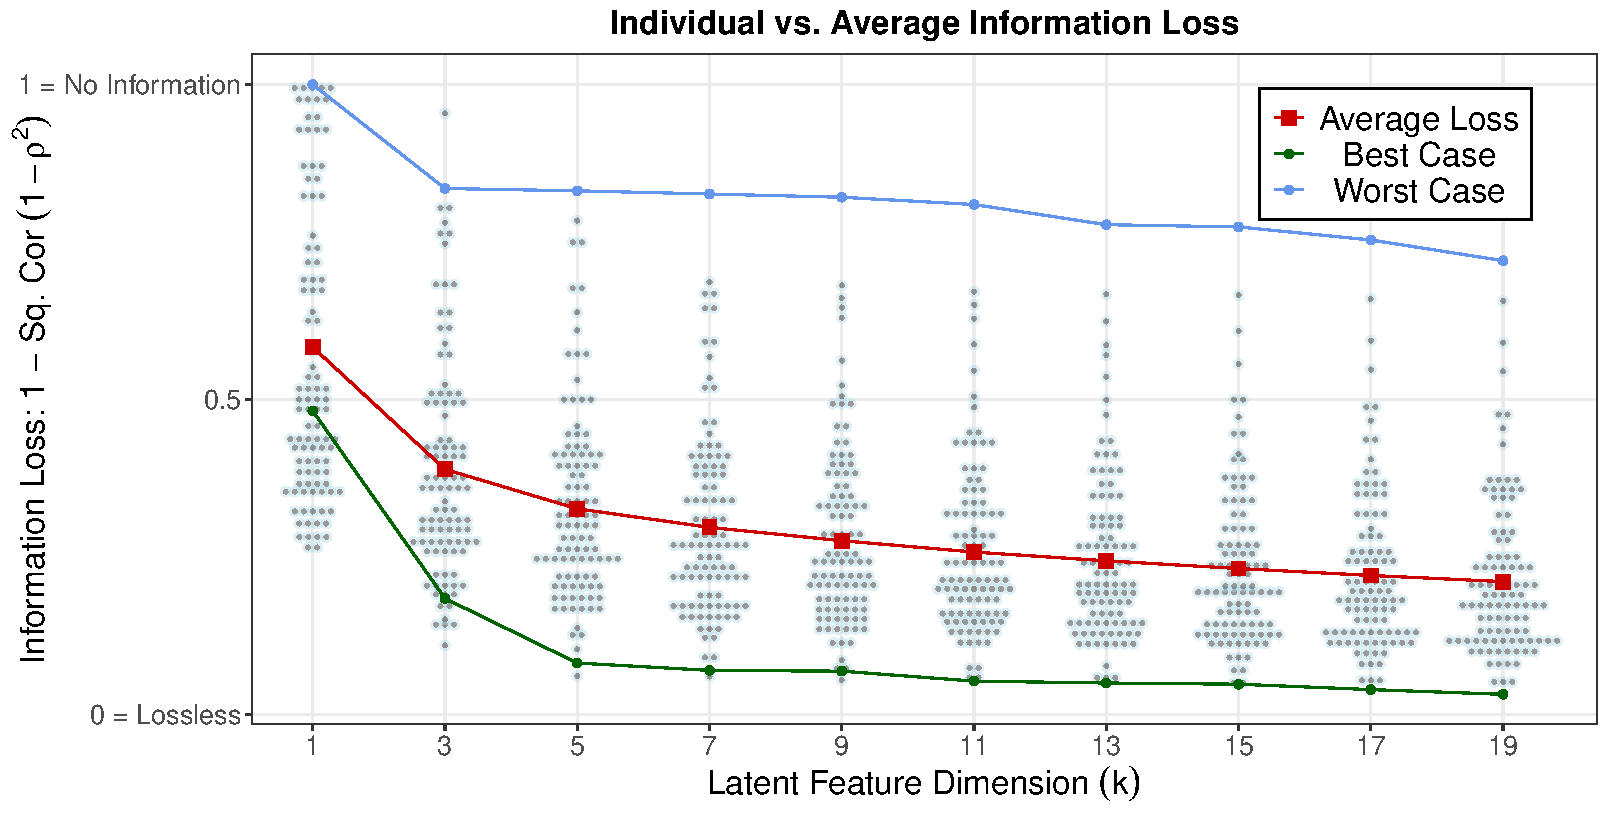
\includegraphics[width=0.75\textwidth]{figures/info-loss.pdf}
    \caption{Generalization errors from a PCA representation of the \texttt{phoneme} data \parencite{hastie_elements_2009}. The grey dots represent individual cross-validated reconstruction errors from PCA representations using different numbers of latent features ranging from $1$ to $19$ ($x$ axis).
    The compliment of the squared correlation is used as reconstruction loss, so $1$ indicates no information retained by the representation and $0$ indicates a lossless representation ($y$ axis).
    The square red points and solid red line trace the average reconstruction error. The green and blue points / lines trace the performance of the best and worst performing observations (selected at $K=19$), respectively.}
    \label{fig:ind-losses}
\end{figure}


Achieving a chosen tolerance level for every observation (i.e., requiring that even the worst case meets the near-losslessness threshold) can sometimes be unrealistic in practice.
Often, a small number of observations (e.g., such as the one traced by the blue points and line in Figure \ref{fig:ind-losses}) possess idiosyncratic features that cannot be captured by a representation that is otherwise compact and near-lossless for the vast majority of the observations.
In this case, using the worst case is overly stringent and results in a latent feature representation that is higher-dimensional and more complex than required for the vast majority of observations.
Therefore, we generalize the notion of near losslessness for the entire dataset, and require it for is met for \emph{quantiles} or \emph{percentiles} of the distribution of individual generalization errors, in which the worst case observation is the $100$th percentile. 
As before, $\epsilon$ denotes the tolerance level of information loss that we want to achieve.
We now introduce the \emph{attainment rate}, which we denote by $\alpha$ as the proportion of observations that we want to achieve this tolerance level.
For example, a attainment rate of $\alpha = 0.95$ would indicate that we require $95\%$ of the observations in the dataset to achieve a loss smaller than the tolerance level $\epsilon$.
We refer to a chosen combination of $\epsilon$ and $\alpha$ as the qualifying criterion and we use the term \emph{qualifying dimension (qd)} to denote the smallest latent feature dimension $K$ for which this criterion is satisfied.
When comparing between two latent feature representation methods (e.g., PCA and autoencoder), for a fixed $\epsilon$ and $\alpha$, we prefer the method with a smaller qualifying dimension as it provides a more compact representation of the dataset.
Finally, we characterize the dimension reduction achieved by a method by its \emph{compression ratio}, which is the ratio of the original data dimension $T$ to the qualifying dimension $qd$, typically rounded to the nearest whole number.

\subsection{Cross-validated Estimation of Information Loss}

Estimating a latent feature representation can equivalently be viewed as a prediction problem, where the goal is to construct $f_{K}$ and $f_{K}^{-1}$ such that the predictions $\widehat{X}_i^{(K)}(\mathbf{t})$ match the observed data $X_i(\mathbf{t})$ as closely as possible \parencite{krzanowski_cross-validation_1987, wold_cross-validatory_1978, diana_cross-validation_2002}.
Hence, it is possible that a latent feature representation method can \emph{overfit} to the data on which it is being learned.
If the information loss of a latent feature representation method is evaluated on that same dataset, then it will tend to be overly optimistic and will not accurately quantify the method's true \emph{generalization error}, which we define as its information loss in reconstructing unseen data.
To obtain a valid estimate of generalization error, it is necessary to use an independent \emph{validation} dataset that is not used to learn the latent feature representation \parencite{diana_cross-validation_2002}.
For example, Figure \ref{fig:training-validation} displays the average information loss in applying PCA to the Proteomic Gels data \parencite{morris_pinnacle_2008} on training and validation sets.
The training set estimate of information loss is overly optimistic and is much lower than the validation estimate.


Generally, with limited data, it is inefficient to perform a single split of the dataset into training and validation sets, as a single random split will tend to be variable (i.e., if the split were performed again, the new validation set would produce a different estimate of information loss) \parencite[Table 1]{collins_evaluation_2024}.
Additionally, because we are interested in the individual values of information loss (rather than an average), sample splitting would only provide us with these values for observations included in the validation set. 
To mitigate these concerns, we employ \emph{cross-validation} \parencite{stone_cross-validatory_1974}, where the data are systematically divided into different training and validation splits, called folds, and the training and validation is performed separately for each split.
When we are interested in an average or total estimate of information loss, cross-validation will tend to be more stable than sample splitting because the estimates are averaged over different folds.
For our purposes, it additionally produces a generalization error estimate for each individual observation in the dataset.
Although cross-validation has long been understood as necessary to estimate generalization error for latent feature representation methods, in particular PCA (e.g., dating back to the work of \textcite{wold_cross-validatory_1978, eastment_cross-validatory_1982, krzanowski_cross-validation_1987}), it is not automatically returned by standard software packages or routinely used in practice to choose between different methods.
Algorithm 1 provides a high-level overview of the full CoLLaRe framework for evaluating latent feature representation methods.





\begin{figure}
    \centering
    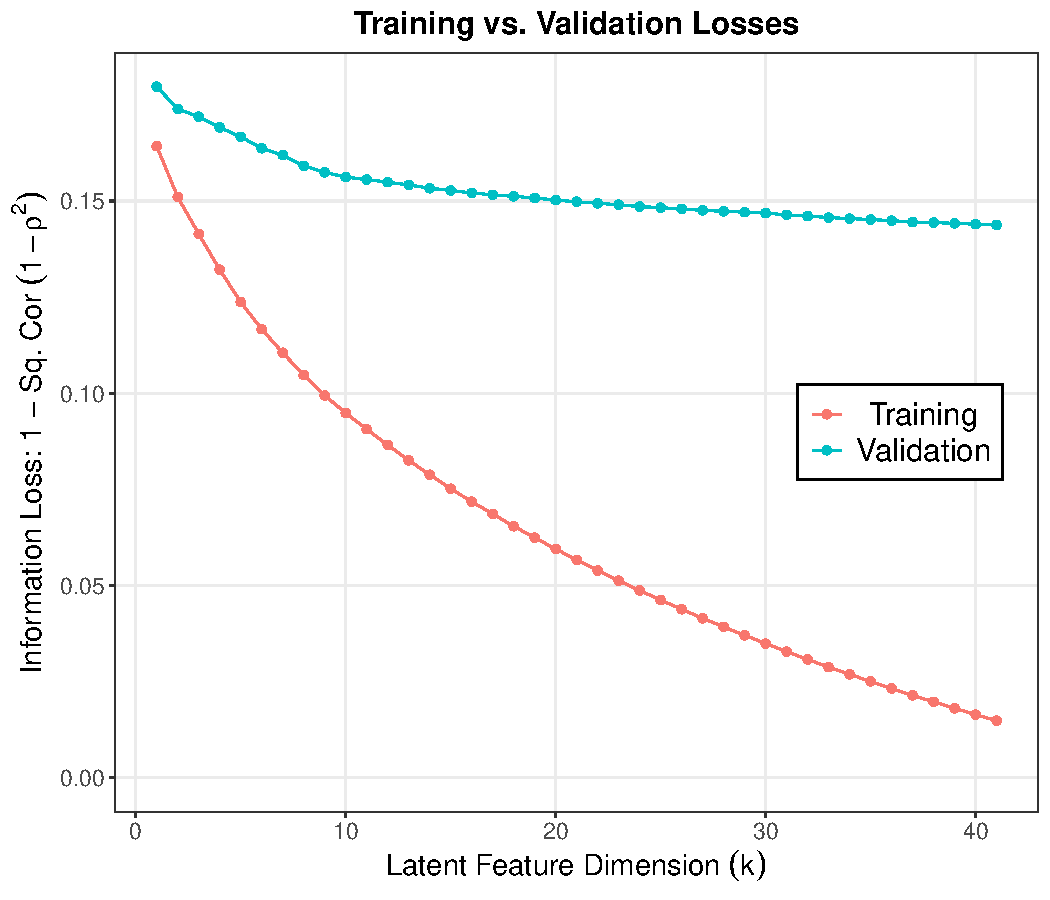
\includegraphics[width=0.5\linewidth]{figures/training-validation.pdf}
    \caption{Example of the average information loss from PCA of the Proteomic Gels data \parencite{morris_pinnacle_2008}, where the loss estimate is computed on the training sample (blue) vs. on a validation sample (red) (i.e., estimated via $5$-fold cross-validation).}
    \label{fig:training-validation}
\end{figure}

\begin{algorithm}
\caption{CoLLaRe Framework for Evaluating Latent Representations}
\begin{algorithmic}[1]

\State \textbf{Initialization} Start with a data matrix $\mathbf{X}$, a latent feature representation method (e.g., PCA, wavelets, or autoencoders) and a choice of loss function. Define the range of latent dimensions to evaluate and the number of folds for cross-validation. Set up a matrix to hold the cross-validated information losses for all observations (in rows) and latent dimensions (in columns).

\State \textbf{Generate cross-validation splits:} Randomly shuffle the dataset and then divide it into training and validation subsets. Reuse these splits across all candidate latent feature dimensions for consistency and efficiency.

\State \textbf{For each candidate latent dimension $K$:}
\begin{enumerate}[a.]
    \item \textbf{For each cross-validation fold:}
    \begin{enumerate}[i.]
        \item \textbf{Train:Validation split:} 
        \begin{itemize}
            \item Split the data into training and validation sets for the current fold.
        \end{itemize}
        \item \textbf{Learn encoding and decoding transformations on training data:}
        \begin{itemize}
            \item Train a representation method (e.g., PCA, wavelets, or autoencoders) on the training data to learn the encoding and decoding transformations $f_K$ and $f^{-1}_K$.
        \end{itemize}
        \item \textbf{Reconstruct validation data:}
        \begin{itemize}
            \item Apply the learned transformations to encode and decode the validation dataset to give reconstructions $\widehat{X}_i (\mathbf{t})$ of $X_i (\mathbf{t})$.
        \end{itemize}
        \item \textbf{Compute information loss on validation data:}
        \begin{itemize}
            \item Measure the dissimilarity between the original and reconstructed validation data for each observation in the validation set using the loss function $g(\cdot, \cdot)$ and store these values.
        \end{itemize}
    \end{enumerate}
\end{enumerate}

\State \textbf{Identify the qualifying dimension:} For each latent dimension, compute the $\alpha$th quantile (e.g., 95th percentile) of the information loss across all observations as specified by the attainment rate $\alpha$. Select the smallest latent feature dimension where this quantile is below the specified tolerance level $\epsilon$.

\State \textbf{Re-train the model at the qualifying dimension:} If a qualifying dimension is identified, re-train the representation method using the full dataset and the qualifying dimension. Store the final trained model for downstream applications.

\State \textbf{Return results:} Return the full matrix of cross-validated information losses and, if applicable, the qualifying latent dimension and the final trained model at that dimension. If applying the algorithm to select among different methods, choose the method with the smallest qualifying dimension.

\end{algorithmic}
\end{algorithm}


